% Chapter 1

\chapter{Introducción} % Main chapter title

\label{Capítulo 1} % For referencing the chapter elsewhere, use \ref{Chapter1} 

%----------------------------------------------------------------------------------------

% Define some commands to keep the formatting separated from the content 
\newcommand{\keyword}[1]{\textbf{#1}}
\newcommand{\tabhead}[1]{\textbf{#1}}
\newcommand{\code}[1]{\texttt{#1}}
\newcommand{\file}[1]{\texttt{\bfseries#1}}
\newcommand{\option}[1]{\texttt{\itshape#1}}
%----------------------------------------------------------------------------------------

\section{Descripción del problema}

La accesibilidad a la bilbiografía de áreas técnicas como la matemática es un tema importante para que la educación sea cada vez más inclusiva.
Aún así, como lo es de importante puede que lo sea de complejo.
En este trabajo se intenta resolver uno de los problemas planteados por alumnos con discapacidades visuales de carreras Licenciatura en Matemática y Licenciatura en Ciencias de la Computación de la Facultad de Matemática Astronomía, Física y Computación, de la UNC.

Uno de los mayores problemas de acceso a la matemática que afecta a la comunidad de estudiantes y científicos ciegos o disminuidos visuales es la lectura de expresiones matemáticas.
El problema es que estas poseen un componente fuertemente visual que se vuelve completamente inaccessible para una persona ciega. \

Este componente visual es la imagen que muestra una expresión matemática, descripta por símbolos especiales que denotan conceptos matemáticos específicos y a veces complejos; por ejemplo, en la fórmula $x \in A \cup B$ encontramos $\in$ y ya sabemos que estamos trabajando con conjuntos y que $x$ es un elemento y $A$ un conjunto, etc. Afortunadamente, esa imagen muchas veces está presente en un archivo pdf y es generada usando \LaTeX{}. Si es un recurso que se puede obtener y manipular, se puede pensar en la accesibilidad.\

La propuesta de solución consiste principalmente en la verbalización de fórmulas matemáticas a partir de expresiones matemáticas escritas en lenguaje \LaTeX{}.
Los sujetos afectados por el problema han encontrado una solución parcial a la accesibilidad de bilbiografía técnica que consiste en utilizar un lector de pantallas (de ahora en adelante ScreenReader) que es un sistema TTS (Text-To-Speach) y su función principal es la lectura en voz alta, a través de un sintetizador de voz, de toda cadena de caracteres presente en la pantalla con el fin de mejorar la accesibilidad.
El inconveniente es que las expresiones matemáticas escritas en \LaTeX{} son leídas literalmente como se muestran y resulta una tarea difícil de comprender para el sujeto que lo esté escuchando.\

Por ejemplo, la siguiente fórmula matemática: \
\textbf{$\frac{1}{2}+\frac{1}{2}=1$} \
que en \LaTeX{} se escribe: \begin{lstlisting}
\frac{1}{2}+\frac{1}{2}=1 \end{lstlisting}
el ScreenReader lee \textbf{\textit{"barra invertida frac uno dos mas barra invertida frac uno dos igual uno"}} mientras que nosotros naturalmente leemos \textbf{\textit{2un medio más un medio es igual a uno"}}.\

Es por eso que este trabajo busca mejorar la accesibilidad de la matemática desarrollando una aplicación que, en un paso previo a la acción del ScreenReader, describa en lenguaje natural las expresiones matemáticas para que luego sean leídas naturalmente.
%----------------------------------------------------------------------------------------

\section{Motivación}

Durante el Censo Nacional de Población, Hogares y Viviendas del año 2010 \cite{1} también denominado Censo del Bicentenario se arrojaron resultados
relativos a la Población con dificultad o limitación permanente (PDLP). En aquel año, Argentina contaba con una población de 39.671.131 de habitantes, de los cuales
5.114.190 habitantes presentaban alguna dificultad o limitación permanente, que representan un 12,9\% sobre el total de la población.
{}
El censo declara en su artículo que se cataloga por discapacitada a toda persona que padezca una alteración funcional permanente o prolongada,
física o mental, que en relación a su edad y medio social implique desventajas considerables para su integración familiar, social, educacional o laboral.\\

\begin{figure}[H]
\centering
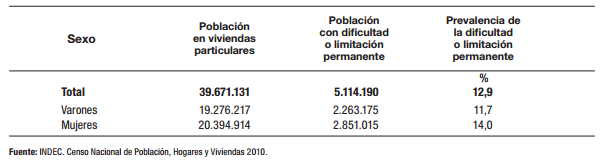
\includegraphics{Figures/porcentaje_discapacitad_por_sexo}
\decoRule
\caption[]{Población con dificultad o limitación permanente y
prevalencia de la dificultad o limitación permanente, por sexo. Año 2010}
\label{fig:porcentaje_discapacitad_por_sexo}
\end{figure}

Concentrándonos en la parte de la población que presenta alguna dificultad visual, el censo obtuvo como resultado que la distribución porcentual
con tal dificultad representa el 59,9\% de la población con dificultades, mientras que el resto de las dificultades (motora superior, motora inferior, cognitiva y auditiva)
se reparten en proporciones casi iguales.

\begin{figure}[H]
\centering
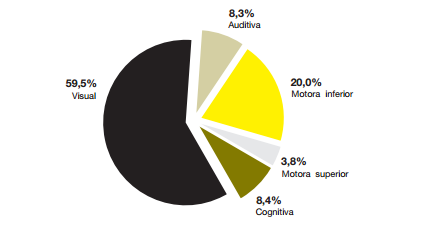
\includegraphics{Figures/poblacion_discapacidad_porcentaje}
\decoRule
\caption[]{Distribución porcentual de la población con una sola dificultad o limitación permanente por tipo de dificultad. Total del país. Año 2010}
\label{fig:poblacion_discapacidad_porcentaje}
\end{figure}

Por lo tanto, la cantidad de personas con discapacidades visuales fue de 3.063.399 en el año 2010. Por otra parte, el 90,2\% de la población concurre
 o concurrió a un establecimiento educativo común, no de educación especial, al que solo fue o va el 9,8 de los encuestados.
 El 26,1\% de los encuestados usa computadora y es la población de entre 6 y 29 años la que más la usa.

La inclusión a la educación es un tema realmente importante para poder incrementar estos números. Aportar a la inclusión ayudará a la población
a insertarse en los distintos niveles educativos.

%---------------------------------------------------------------------------------------

\section{Alcance de la tesis}

Se desea construir una prueba de concepto, que llamaremos \textit{TexToES},  que intente resolver el problema planteado.
TexToES podrá procesar los siguientes tipos diferentes de entradas:
\begin{itemize}
\item una expresión matemática escrita en \textbf{\LaTeX{}},
\item una expresión matemática escrita en \textbf{MathML},
\item \textbf{archivo} que contenga expresiones matemáticas escritas en \LaTeX{}.
\end{itemize}
Dada cualquiera de estas entradas, la PoC hará traducción al lenguaje natural en español de las expresiones matemáticas y será devuelto en texto.
Además, la PoC asumirá la existencia de un convertor de LaTeX a MathML (adelante en este trabajo se explicará la necesidad de este componente) y no generará TTS. \
Con el objetivo de hacer este trabajo lo más flexible posible, TexToES busca que funcione modularmente entre las distintas entradas y el sistema TTS preferido por el usuario.

%---------------------------------------------------------------------------------------

\section{Estructura de la tesis}

El siguiente trabajo de tesis se divide en cinco secciones principales. En la sección 1  se menciona una introducción al trabajo de tesis, se brinda una idea introductoria del problema que la tesis busca resolver. A su vez, esta sección busca dar un contexto social al problema y destacar la importancia de su solución. Además se busca definir qué alcance tendrá el trabajo y su proyecto asociado.

En la sección 2 \textit{- Análisis de tipos de entrada -} se muestra un análisis de cómo encarar el problema que se quiere resolver, mostrando qué tipos de entradas son las que manipulan los sujetos involucrados. También, esta sección busca desarrollar con el lector los términos y las definiciones que serán utilizados a lo largo del documento, conocer en detalle qué ofrece y qué no ofrece cada entrada. Finalmente, muestra los argumentos que llevan a la decisión de cómo iniciar el proceso de desarrollo de la solución.

En la sección 3, \textit{Arquitectura de la solución}, se muestra al lector cuáles partes están involucradas y que conjuntamente forman a la solución final. Esta seccion define los distintos alcances, objetivos, acciones, comportamientos de cada componente. A su vez, quiere describir la manera en la que estos componentes se comunican.

En la sección 4, \textit{Construcción y evaluación de la gramática}, se indican los mecanismos empleados para la construcción de este verbalizador, que busca mejorar la accesibilidad de la matemática y, a su vez, se muestran tres maneras de evaluar el verbalizador. El objetivo de esta sección es poder mostrar cómo el verbalizador puede mejorar para que se asemeje cada vez más a como nosotros mismos dictaríamos una expresión matemática a una persona que no puede verla.

Finalmente, si bien los anexos no son una sección en particular, aquí está presente toda la evidencia que el resto del trabajo cita y en la cual se basa. Intenta que el lector tenga más contexto si desea averiguar un poco más acerca de lo que está leyendo.
